\section{Overview de modelos}

\begin{frame}	
	\begin{block}{Modelos}	
			\begin{figure}[!htb]
			\centering	  				
			
\includegraphics[height=6cm, width = 10cm]{./pic/AI.png}
			\caption{Brincadeira, cada modelo trabalha internamente de uma forma distinta!}
			\label{fig_brincadeira}
		\end{figure}	
	\end{block}
\end{frame}

\begin{frame}	
	\begin{block}{Modelos}	
		\begin{itemize}
			\item Modelos tomam decisões baseados em diversas variáveis para, entre outras coisas, classificar dados
			\item Quem são peruanos e quem são brasileiros nessa sala?
			\item Há modelos para classificar em duas classes ou mais.
		\end{itemize}			
		\begin{figure}[!htb]
			\centering	  				
			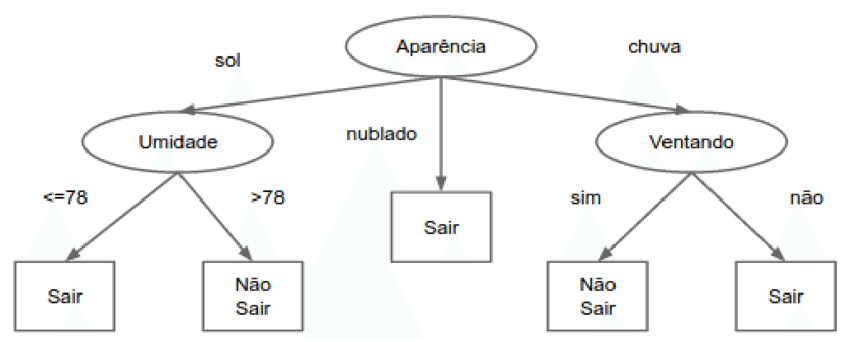
\includegraphics[height=4cm, width = 10cm]{./pic/arvore.png}
			\caption{Exemplo de árvore de decisão para sair de casa}
			\label{fig_Arvore}
		\end{figure}	
	\end{block}
\end{frame}